\documentclass[dvips]{radhazu}
\usepackage{radhazu}
\usepackage{graphicx}
%\usepackage[T1]{fontenc}
%Additional packages if necessary
%\usepackage{epsfig,amscd,amssymb,amsxtra,amsmath,amsthm}




%the following line resets the counter of the equations at the beginning of the sections
%\def\SectionNumberingEquation{\setcounter{equation}{0}}

%the following two lines set the line numbers
%\usepackage[pagewise]{lineno}
%\pagewiselinenumbers

%ignore the next few lines (delete them in your paper)
\begin{filecontents*}{example.eps}
%!PS-Adobe-3.0 EPSF-3.0
%%BoundingBox: 19 19 121 121
%%CreationDate: Thu Feb 06 2003
%%Creator: programmed by hand
%%EndComments
gsave newpath
  20 20 moveto
  20 120 lineto
  120 120 lineto
  120 20 lineto
closepath
    2 setlinewidth
gsave
    0.8 setgray fill
grestore
    stroke
grestore
\end{filecontents*}




\begin{document}


\title[Running title]{Title}

\author[F. Author, S. Author and L. Author]{First author, Second author and Last author}
\address[First author]{Department of Mathematics\\University of Zagreb\\ 10 000 Zagreb, Croatia}
\email[First author]{First@math.hr}

\address[Second author]{Department of Mathematics\\University of Zagreb\\ 10 000 Zagreb, Croatia}
\email[Second author]{Second@math.hr}

\address[Last author]{Department of Mathematics\\University of Zagreb\\ 10 000 Zagreb, Croatia}
\email[Last author]{Last@math.hr}


\keywords{template, \LaTeX style}

\subjclass{?????, ?????}



\abstract{Enter your abstract here.}



\maketitle

\section{Introduction}
\label{intro}

Your text comes here. Separate text sections with

\section{Section title}
\label{sec:1}
 \ and

\subsection{Subsection title}
\label{sec:2}

as required. Don't forget to give each section and subsection a
unique label (see Sect.~\ref{sec:1}).

\section{Environments}

The following environments are predefined:
\begin{theorem}\label{thm:1}
Text
\end{theorem}
\begin{proof}
Proofs of theorems and such should end with a square.
\end{proof}
\begin{corollary}\label{cor:1}
Text
\end{corollary}
\begin{conjecture}\label{con:1}
Text
\end{conjecture}
\begin{lemma}\label{lem:1}
Text
\end{lemma}
\begin{proposition}\label{pro:1}
Text
\end{proposition}
\begin{axiom}\label{axi:1}
Text
\end{axiom}
\begin{exercise}\label{exe:1}
Text
\end{exercise}
\begin{problem}\label{prob:1}
Text
\end{problem}
\begin{definition}\label{def:1}
Text
\end{definition}
\begin{example}\label{exa:1}
Text
\end{example}
\begin{remark}\label{rem:1}
Text
\end{remark}
Don't forget to label environments (see Theorem~\ref{thm:1},
\ldots, Remark~\ref{rem:1}).

\section{Mathematical formulae}

For unnumbered mathematical formula use
$$%\[
y=x.
$$%\]
For numbered mathematical formula use
\begin{equation}\label{eq:1}
x=z.
\end{equation}
For multiline formulae use
\begin{align}
&y=x,\\
&x=z. %\nonumber    %uncomment for unnumbered formula
\end{align}
To refer on formulae use the notation (\ref{eq:1}).

\section{Figures and tables}

For figures use
\begin{figure}[ht]
\begin{center}
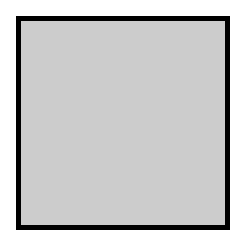
\includegraphics[width=0.3\textwidth]{example.eps}
\caption{Please write your figure caption here}
\label{fig:1}       % Give a unique label
\end{center}
\end{figure}

For \LaTeX tables use
\begin{table}[ht]
\caption{Please write your table caption here}
\label{tab:1}       % Give a unique label
\begin{tabular}{lll}
\hline
first & second & third  \\
\hline
number & number & number \\
number & number & number \\
\end{tabular}
\end{table}


\Acknowledgements{If necessary your acknowledgements enter here.}



The references should be arranged and numbered in alphabetical
order, referred by \cite{agatutekveselic} or \cite{tadic} and
cited as follows:

\begin{thebibliography}{99}

\bibitem{agatutekveselic}{I.~Aganovi\'c, Z.~Tutek and K.~Veseli\'c,}
\textit{Approximation of Green's function and application,}
Glas.~Mat.~Ser.~III \textbf{35(55)} (2000), 179--190.

\bibitem{bestvinahandbook}{M.~Bestvina,}
\textit{$\Bbb R$-trees in topology, geometry, and group theory,}
in: Handbook of geometric topology (eds. R.~J.~Daverman and
R.~B.~Sher), North-Holland, Amsterdam, 2002, 55--91.

\bibitem{bestvinapaper}{M.~Bestvina and K.~Fujiwara,}
\textit{Bounded cohomology of subgroups of mapping class groups.}
Geom.~Topol.~\textbf{6} (2002), 69--89 (electronic).

\bibitem{brailo}{Yu.~A.~Brailov,}
\textit{The topology of bifurcation diagrams of integrable systems
on semisimple Lie algebras,} Dokl.~Akad.~Nauk~\textbf{375} (2000),
151--153 (in Russian).

\bibitem{brezis}{H. Brezis,} Analyse fonctionnelle. Th\'{e}orie
    et applications, Masson, Paris, 1983.

\bibitem{mardesicproceedings}{S.~Marde\v{s}i\'{c},}
\textit{Shape fibrations for topological spaces}, in: Shape theory
and topological spaces (ed. Y.~Kodama), Proc. of the Research
Institute for Math.~Sci.~445, Kyoto 1981, 15 - 18.

\bibitem{mardesicpaper}{S.~Marde\v{s}i\'{c},}
\textit{Nonvanishing derived limits in shape theory},
Topology~\textbf{35} (1996), 521-532.

\bibitem{mardesic}{S.~Marde\v{s}i\'{c} and J.~Segal,}
Shape Theory, North-Holland, Amsterdam, 1982.

\bibitem{tadic}{M.~Tadi\'c,}
\textit{On square integrable representations of classical $p$-adic
groups}, preprint.
\end{thebibliography}

\bigskip

\bigskip

\begin{center}
{\bf Naslov}
\end{center}

\bigskip

\begin{center}
{\it Prvi autor, drugi autor i tre\'ci autor}
\end{center}

\bigskip

\begin{center}
\begin{minipage}[c]{9.2cm}
{\small \hspace*{0.5cm} {\sc Sa\v{z}etak.}
Hrvatski prijevod sa\v{z}etka.}%
\end{minipage}
\end{center}

\endarticle 

\end{document}
